\chapter{\twor}\label{two}

\begin{wrapfigure}{l}{0.05\textwidth}

\includegraphics[width=\linewidth]{logo_1}
\label{fig:wrapfig}
\end{wrapfigure}

\paragraph{What is it?} The \twor\  is a malicious Android application masquerading as a plugin for a transportation application series developed by a South Korean developer. The series provides a range of information for each region of South Korea, such as bus stop locations, bus arrival times and so on.
    \section{VirusTotal}
        \begin{figure}[h]
            \centering
            
\includegraphics[width=1\linewidth]{virustotal_2_summary.png}
            \caption{Virustotal summary analysis of file \twor}
            \label{fig:virustotal_1_summary}
        \end{figure}
        \subsection{Detection}
        \begin{figure}
            \centering
        
\includegraphics[width=\linewidth]{virustotal_2_detection_complete.png}
            \caption{VirusTotal Detection tab for \twor}
            \label{fig:virustotal_2_detection_comp}
        \end{figure}
        The antimalware analysis performed with VirusTotal, shown in fig. \ref{fig:virustotal_1_detection_comp}, highlights that:
        \begin{itemize}
            \item 40 out of 76 security vendors flagged the file as "\textbf{malicious}";
            \item 29 out of 76 security vendors flagged the file as a "\textbf{secure file}";
            \item 7 out of 76 security vendors get a "\textbf{Unable to process file type}" error
        \end{itemize}
        
        Most anti-malware programs correctly identify the sample as a generic android trojan, but some of them are even able to recognize its malware family (downloader). 
        A few vendors classify the sample as a generic android malware, without specifying the family nor the type (trojan).\\
        It’s interesting to notice that some famous vendor like Microsoft Defender, McAfee and Malwarebytes were unable to identify the file as malicious.
         \clearpage
        \subsection{Details}
        \begin{figure}[h]
            \centering
            
\includegraphics[width=.5\linewidth]{virustotal_second_permissions.png}
            \caption{Android Permission of \twor}
            \label{fig:virustotal_second_permissions}
        \end{figure}
            The detailed analysis of the permissions (Fig. \ref{fig:virustotal_second_permissions}) which are required by the APK, declared in the Manifest file (Fig. \ref{fig:manifest_second}) is skipped since it's similar to the previous one done on \ref{sec:perm_analysis}.
    \begin{figure}[h]
        \centering
        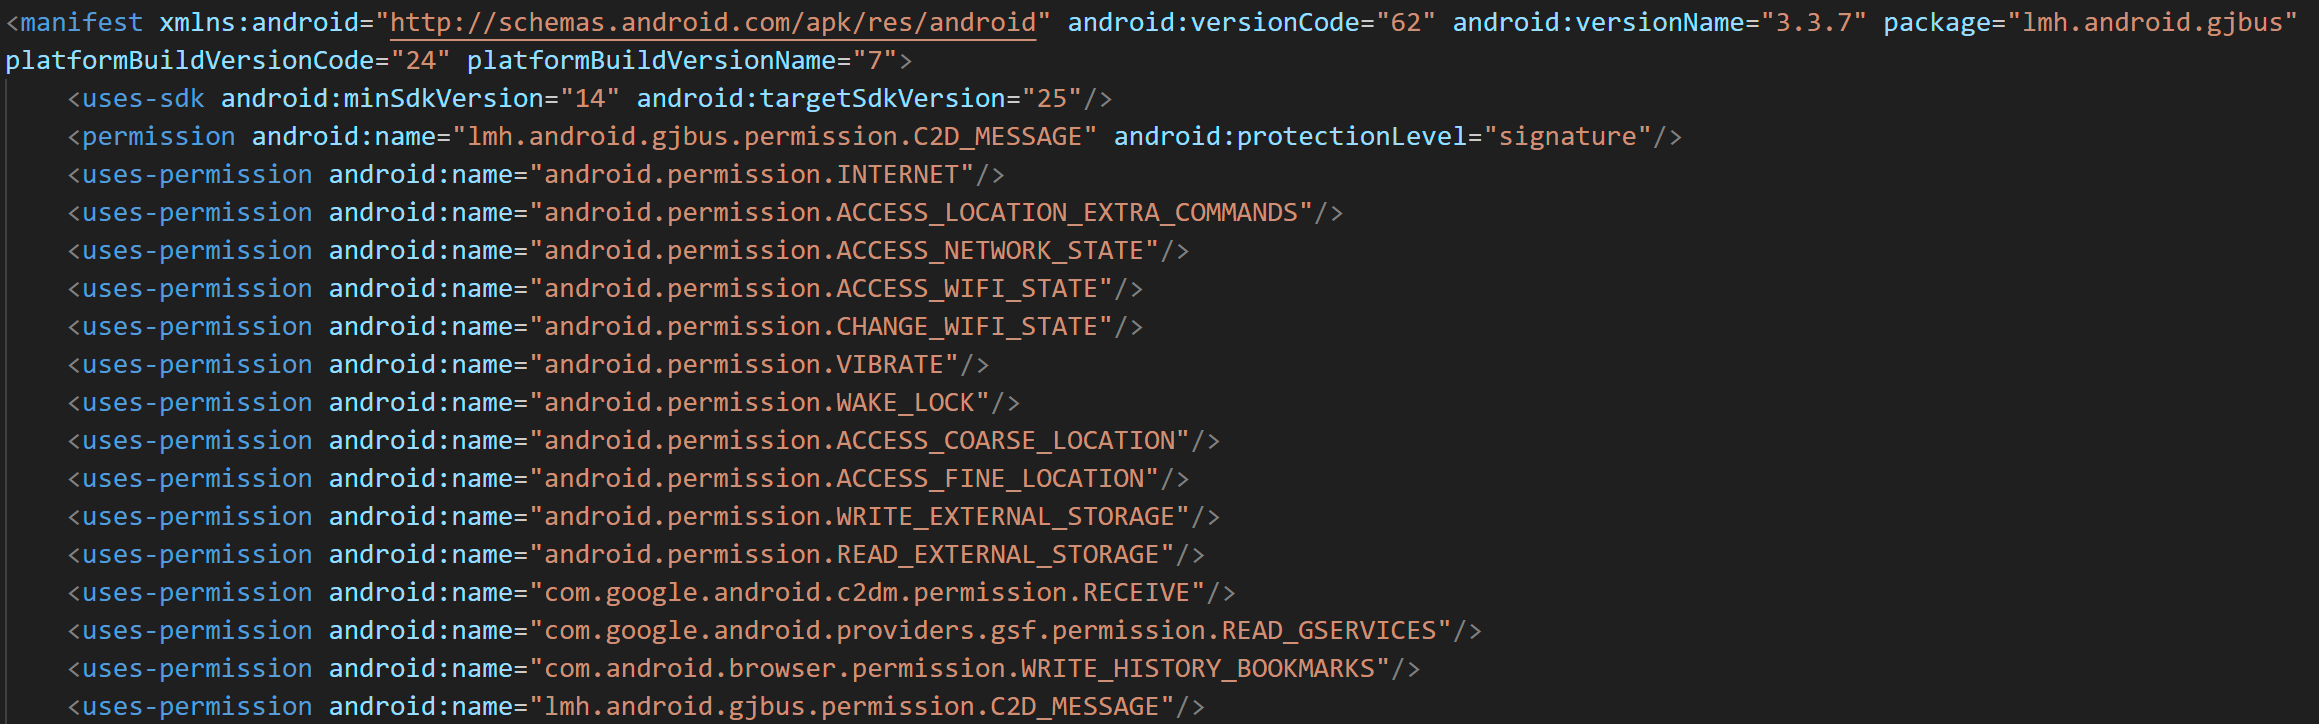
\includegraphics[width=\linewidth]{img/manifest_second.png}
        \caption{Android Manifest \twor}
        \label{fig:manifest_second}
    \end{figure}
            
        \subsection{Relations}
        \begin{figure}[h]
            \centering
            \includegraphics[width=1\linewidth]{second_realtions.png}
            \caption{Enter Caption}
            \label{fig:virustotal_2_relations}
        \end{figure}
         In Fig. \ref{fig:virustotal_2_relations} are showed the contacted domains, URLS and IP that are contacted by the malware APK.
         The first three URLs are hosted by AWS Elastic Beanstalk and they act to retrieve the category, the environment and the issue from a central database; while the last one seems to retrieve a configuration init file to show advertisement.
         Therefore, the \link{busappmanager.elasticbeanstak.com} website is currently \underline{unavailable}, while the \link{gwk.adlibr.com/ad/config/init} is UP and requires a POST requests otherwise it returns the following json response: \begin{CJK*}{UTF8}{mj}
         \texttt{\{"result": 4003,"message": "key media key} 필수입니다."\}
         \end{CJK*} (the translate response message says: "key media key is required").
            \todo[inline]{Add more information about Relations tab}
        \subsection{Behavior}
            \todo[inline]{Add more information about Behavior tab}
        
    \section{Static Analysis}
    
\subsection{MainActivity.java}
\begin{itemize}
  \item Inherits from \texttt{BaseMainActivity}
  \item Calls \texttt{getTabView(BaseTabFragmentActivity.MainTabs.BUSTRANS).setVisibility(8)} to hide a UI tab
  \item Provides AD network keys through \texttt{getAdvertiseKey(...)}
  \item Retrieves configuration via \texttt{getEnvironmentProperties(...)}
\end{itemize}
\textbf{Suspicion:}
\begin{itemize}
  \item UI obfuscation suggests conditional behaviors
  \item Uses multiple AD providers (AdMob, Facebook, AdLib)
\end{itemize}

\subsubsection{BaseMainActivity.java}
\begin{itemize}
  \item Central logic hub for initialization
  \item Loads native library: \texttt{System.loadLibrary("Audio3.0")}
  \item Declares and invokes native methods: \texttt{startUpdate()} and \texttt{updateApplication()}
  \item Requests runtime permissions:
    \begin{itemize}
      \item \texttt{READ/WRITE\_EXTERNAL\_STORAGE}
      \item \texttt{REQUEST\_INSTALL\_PACKAGES}
    \end{itemize}
  \item Loads remote app environment with URL, DB version, and remote download URL
\end{itemize}
\textbf{Critical:}
\begin{itemize}
  \item Behavior consistent with droppers
  \item Remote configuration allows behavior change without app update
\end{itemize}

\subsection{EnvConstant.java}
\begin{lstlisting}[language=Java]
public static final String ADAM_KEY = "3034Z1OT1385cf1db09";
public static final String ADLIB_KEY = "590ea88a0cf2843c93807ed9";
public static final String ADMOB_UNITID = "ca-app-pub-0388605861855854/7499990747";
public static final String FACEBOOK = "627046304133735_685335228304842";
public static final String GA_TRACKER_ID = "UA-56668425-6";
\end{lstlisting}

\textbf{Observation:}
\begin{itemize}
  \item Multiple ad SDKs used aggressively
  \item No endpoint URLs found here directly, but likely part of environment loading
\end{itemize}

\subsection{BusApiWeb.java}
\begin{itemize}
  \item Makes calls to:
    \begin{itemize}
      \item \texttt{http://bus.changwon.go.kr/busInfo/busInfoDetail.jsp}
      \item \texttt{http://bus.changwon.go.kr/busInfo/mapLayer.jsp}
    \end{itemize}
  \item Uses Volley for networking
  \item Parses HTML responses (not JSON)
  \item Relays info through listeners
\end{itemize}
\textbf{Issue:}
\begin{itemize}
  \item HTTP-only communication
  \item Bus stop and route IDs travel in plaintext
  \item High risk of MITM
\end{itemize}

\subsection{AndroidManifest.xml}
\begin{itemize}
  \item Declares permissions:
    \begin{itemize}
      \item INTERNET, LOCATION (fine \& coarse), READ/WRITE\_STORAGE, INSTALL\_PACKAGES
    \end{itemize}
  \item Declares multiple ad and analytics activities:
    \begin{itemize}
      \item AdLib, AdMob, Facebook, AdFit (Kakao)
    \end{itemize}
  \item GCM and Firebase messaging
  \item Custom Service: \texttt{lmh.android.cwbus.GCMIntentService}
\end{itemize}
\textbf{Observations:}
\begin{itemize}
  \item App declares capability to receive background messages
  \item May be used to trigger behavior remotely
  \item Can install new APKs silently if permissions are granted
\end{itemize}

\subsection{AppInfoActivity.java}
\begin{itemize}
  \item Displays a link: \texttt{http://bus.changwon.go.kr/main}
  \item Serves to legitimize the app
  \item No interaction logic
\end{itemize}
\textbf{Note:} Used to present legitimacy but exposes HTTP link

\section{Summary}

\begin{longtable}{|p{0.45\textwidth}|p{0.45\textwidth}|}
\hline
\textbf{Suspicious Pattern} & \textbf{Explanation} \\
\hline
Multiple Ad SDKs & Monetization via ad fraud or over-advertising \\
\hline
Native Libraries (JNI) & Executes code not visible to static tools, common in evasion \\
\hline
Request Install Packages & Dropper-like behavior: installs APKs without market interaction \\
\hline
Unencrypted HTTP endpoints & Data exposed to interception (MITM) \\
\hline
Dynamic config via EnvProperties & App changes behavior based on remote values \\
\hline
Fragment and tab visibility manipulation & Delays/masks functionality from user and analysts \\
\hline
\end{longtable}

\subsection{Conclusion}

This app contains multiple suspicious behavior, including installation of APKs via native code, aggressive ad loading, and unencrypted network activity. It appears to be built on a legitimate transport-use-case shell but may act as a secondary payload installer.
    \section{MobSF}
    During the performed analysis, have been found 1 unique certificate:
    \begin{itemize}
        \item[] Binary is signed
        \item[]v1 signature: True
        \item[]v2 signature: False
        \item[]v3 signature: False
        \item[]v4 signature: False
        \item[]X.509 Subject: C=ko, L=Jeonju, CN=Myoung-Hun Lee
        \item[]Signature Algorithm: rsassa\_pkcs1v15
        \item[]Valid From: 2011-05-25 07:49:38+00:00
        \item[]Valid To: 2061-05-12 07:49:38+00:00
        \item[]Issuer: C=ko, L=Jeonju, CN=Myoung-Hun Lee
        \item[]Serial Number: 0x4ddcb492
        \item[]Hash Algorithm: sha1
        \item[]md5: f30f4a17918f7e5f0ea983342c58b383
        \item[]sha1: e849315f29e8049a7c865b22367b3fc75a1c132b
        \item[]sha256: 0c50896699e9f7bb3c1a3ed75fa6a636b791d29b635c89d2deb1fa8f46fd2c2d
        \item[]sha512: 77654172411f3e08ea714f4032ab0c32438c921c134288cff30fcd2c8a7ba174de3dd95579cf76ffaabc8e578bf5a37b234e042862266a0d46e3b0ae053cf2f6
    \end{itemize}
    \begin{figure}[h]
        \centering
        
\includegraphics[width=\linewidth]{mobsf_two_scorecard.png}
        \caption{MobSF Application Security Scorecard \twor}
        \label{fig:mobsf_scorecard_two}
    \end{figure}
    As showing in Fig. \ref{fig:mobsf_scorecard_two}, the app presents the following issue, grouped by severity:
    \begin{itemize}
        \item High (9) $\rightarrow$ , which have a significant impact on the privacy of the user. The problem are:
        \begin{enumerate}
            \item Application vulnerable to Janus Vulnerability, due to the version of the signature scheme used; the vulnerability is present on Android 5.0-8.0 if signed only with v1 signature schema;
            \item  Certificate algorithm vulnerable to hash collision, the APK is signed using SHA1withRSA which is known to have a collision issues generating the same hashes for different files;
            \item  App can be installed on a vulnerable unpatched Android, on the Manifest file the minimum SDK version is set to be 14, this may lead the app to be installed on older devices with unfixed vulnerabilities;
            \item \label{standhoogg} lmh.android.cwbus.activity.AlarmActivity vulnerable to Android Task Hijacking/StrandHogg, resulting in the possibility of other applications to place a malicious activity on top of the activity stack resulting in the above vulnerability;
            \item  Activity (com.google.android.gms.appinvite.PreviewActivity) is vulnerable to StrandHogg 2.0, similar to finding \ref{standhoogg};
            \item Debug configuration enabled,Production builds must not be debuggable;
            \item Weak Encryption algorithm used on adlib library (com/mocoplex/adlib/util/b.java, line(s) 20)
            \item The file or SharedPreference is World Readable. Any App can read from the file, the file in question is \textit{ com/mocoplex/adlib/dlg/b.java, line(s) 148}
            \item  Application contains Privacy Trackers, it has more than 8 privacy trackers, which track device or users and are privacy concerns for end users.
        \end{enumerate}
        \item Medium (21) $\rightarrow$ \begin{enumerate}
            \item The string $[android:allowBackup=true]$, allows anyone to backup the application data via adb if USB debugging is enabled
            \item Launch Mode of activity (lmh.android.cwbus.activity.AlarmActivity) is not standard, an Activity should not be having the launch mode attribute set to "singleTask/singleInstance" because it may becomes root Activity and any other applications can read the contents of the "calling Intent";
            \item \label{br} The string $[android:exported=true]$, a broadcast receiver is found to be shared with other apps leading to be accessible to any other app on the device;
            \item \label{pl} The broadcast receiver seen in \ref{br} is protected by an external permission, leading to not be scanned to check the effective protectionLevel;
            \item The presence of intent-filter indicates that the Activity (com.kakao.adfit.common.inappbrowser .activity.IABActivity) is explicitly exported;
            \item com.google.android.gms.appinvite.PreviewActivity) is not Protected, same as \ref {br}
            \item Permission: com.google.android.gms.auth.api.signin.permission.REVOCATION\_NOTIFICATION, presents the same permission protection level as \ref{pl}
            \item Service (com.google.firebase.messaging.FirebaseMessagingService) is not Protected, as \ref{br}
            \item  Activity (com.google.android.gms.tagmanager.TagManagerPreviewActivity) is not Protected, as \ref{br}
            \item Broadcast Receiver (com.google.android.gms.measurement.AppMeasurementInstallReferrerReceiver) is Protected by a permission, but the protection level of the permission should be checked, with the permission android.permission.INSTALL\_PACKAGES, same as \ref{pl}
            \item Broadcast Receiver (com.google.firebase.iid.FirebaseInstanceIdReceiver) is Protected by a permission, but the protection level of the permission should be checked, with permission com.google.android.c2dm.permission.SEND, should be check as \ref{pl}
            \item Service (com.google.firebase.iid.FirebaseInstanceIdService) is not Protected, as \ref{br}
            \item App can read/write to External Storage, consequently any other app on the device can read data written to External Storage
            \item Files may contain hardcoded sensitive information like usernames, passwords and keys, founded in the following files:
            \begin{itemize}
                \item com/kakao/adfit/publisher/BuildConfig.java, line(s) 9
                \item com/kakao/adfit/publisher/impl/AdCommon.java, line(s) 10
                \item com/mocoplex/adlib/AdlibConfig.java, line(s) 505
                \item com/mocoplex/adlib/platform/c.java, line(s) 227,293
                \item lmh/android/cwbus/api/BusApiXml.java, line(s) 22
                \item lmh/android/cwbus/constants/EnvConstant.java, line(s) 5,6
                \item org/jsoup/helper/W3CDom.java, line(s) 55
                \item org/jsoup/nodes/Comment.java, line(s) 8
                \item org/jsoup/nodes/DataNode.java, line(s) 8
                \item org/jsoup/nodes/DocumentType.java, line(s) 12,13,15
                \item org/jsoup/nodes/TextNode.java, line(s) 10
            \end{itemize}
            \item Using MD5 which is a weak hash known to have collisions;
            \item Insecure WebView Implementation. Execution of user controlled code in WebView is a critical Security Hole, in the file \textit{com/mocoplex/adlib/dlg/AdlibDialogView.java, line(s) 91,113,85,110}
            \item App creates temp file, which reveals sensitive information which should never be written into file.
            \item The App make uses of an insecure Random Number Generator
            \item Enabling file access from URLs in WebView can leak sensitive information from the file system.
            \item App uses SQLite Database and execute raw SQL query. Untrusted user input in raw SQL queries can cause SQL Injection. Also sensitive information should be encrypted and written to the database.
            \item App contains hardcoded secrets.
        \end{enumerate}
        \item Info (1) $\rightarrow$ \begin{enumerate}
            \item The App logs information, including sensitive information which should never be logged.
        \end{enumerate}
        \item Secure (2) $\rightarrow$ \begin{enumerate}
            \item The app uses SSL certificate due to detect or prevent MITM attacks using secure communication channel
            \item The app have root detection capabilities
        \end{enumerate}
        \item Hotspot (1) $\rightarrow$ critical permission found
    \end{itemize}
            \todo[inline]{Add MobSF malware analysis}
    \section{Genymotion}
            \todo[inline]{Add Gennymotion malware analysis}
        